% *********************** Це є Розділ 2 ************************************

 \markright{\underline {\it Розділ 2. Теоретичне рішення проблеми}}

 \setcounter{chapter}{1}
 \chapter{Теоретичне рішення проблеми}

 
 У цьому розділі буде описано теоретичне рішення проблеми глибокого навчання з 
 підкріпленням (DRL), зокрема, розглянемо три основні алгоритми DRL, які широко 
 використовуються у відеоіграх: Deep Q-Network (DQN), Advantage Actor-Critic (A2C) 
 та Proximal Policy Optimization (PPO). Кожен з цих алгоритмів має свої особливості, 
 переваги та обмеження, що робить їх застосування ефективним у різних сценаріях.
 Крім того, розглянемо проблему представлення ігрового середовища 
 для алгоритмів DRL. Для ефек\-тив\-ного навчання алгоритми повинні отримувати 
 відповідні, добре структуровані дані про стан ігрового середовища. Це включає 
 обробку зображень, що надають інформацію про поточний стан гри, та перетворення 
 їх у форму, придатну для обробки нейронними мережами. Також важливим є вибір метрик 
 і винагород, які б точно відображали цілі та прогрес у грі, щоб алгоритми могли 
 ефективно вчитися і приймати оптимальні рішення.

\section{Навчання з підкріпленням (RL)}
  \setcounter{equation}{0}
 \setcounter{theorem}{0}
 \par  Традиційно RL використовує математичні алгоритми для моделювання та 
  визначення винагороди на основі невеликих наборах даних та простому навколишньому
  середовища. Ця проблема часто моделюється ма\-те\-ма\-тич\-но як {\em марковський процес 
  вирішування}. Марковський процес вирішування (МПВ) - 
  це стохастичний процес прийняття рішень, який використовує математичний 
  апарат для моделювання прийняття рішень динамічною системою. 
  Він використовується в сценаріях, де результати або випадкові, або 
  контролюються особою, яка приймає послідовні рішення в 
  часі. МПВ оцінює, які дії має здійснити особа, що приймає рішення, з огляду
  {\em лише на поточний стан середовища}. Зрозуміло, що якщо дія агента залежатиме від 
  усіх попередніх станів та дій це призведе де неймовірної комплексності задачі. Тому 
  функ\-ція переходу набуває наступного вигляду:
  \bql{eq:shortstatedistribution}
  s_{t+1} \sim P(s_{t+1} \vert s_{t}, a_{t}),
  \eq
  \\ де $s_{t}$, $a_{t}$ - стан системи та дія агента  на кроці $t$.
  \par Тепер МПВ може бути сформульований у контексті RL. МПВ визначається
  кортежом з 4-х елементів, $(\EuScript{S, A}, P(.), \EuScript{R(.)})$, де
  \begin{itemize}
    \item $\EuScript{S}$ - множина станів. 
    \item $\EuScript{A}$ - множина дій. 
    \item $P(s_{t+1} \vert s_{t}, a_{t})$ - функція переходу станів середовища.
    \item ${\EuScript{R}(s_t,a_t,s_{t+1})}$ - функ\-ція винагороди середовища.
  \end{itemize} 
  Одне з важливих припущень, що лежить в основі проблем навчання з підкріпленням, полягає в тому, 
  що агенти не мають доступу до функції переходу $P(s_{t+1} \vert s_{t}, a_{t})$ або функції винагороди 
  ${\EuScript{R}(s_t,a_t,s_{t+1})}$. Єдиний спосіб, яким агент може отримати інформацію про ці функції це через
  стани, дії та винагороди, які він отримує досліджуючи навколишнє середовище, тобто кортежі "досвіду" $(s_t, a_t, r_t)$.
  {\em Тракеторією} будемо називати послідовність отриманого агентом досвіду на протязі одного епізоду, тобто 
  $\tau = (s_0,a_0,r_0),\dots,(s_t,a_t,r_t)$
  \par Щоб завершити формулювання задачі, нам також потрібно формалізувати поняття цілі, яку максимізує агент. 
  Спочатку визначимо прибуток $R(\tau)$ використовуючи траекторію з епізоду: \bql{eq:return}   R(\tau) = r_0 + \gamma r_1 + \gamma^2 r_2 + \dots + \gamma^{k} r_k = \sum_{t=0}^{k} \gamma^t r_t.\eq
 \par Рівняння \ref{eq:return} визначає прибуток як суму винагород, де $\gamma \in [0,1]$ - коефіцієнт знижки.
 \par Тоді означемо так звану {\em ціль} $J(\tau)$ яка є просто сподіванням прибутковості за багатьма траєкторіями, як показано в рівнянні \ref{eq:objective}:
 \bql{eq:objective} J(\tau) = \EX_{\tau \sim \pi}[R(\tau)] = \EX[\sum_{t=0}^{k} \gamma^t r_t]. \eq
 \par Прибуток $R(\tau)$ - це сума знижених винагород $\gamma^t r_t$ на всіх часових кроках $t = 0,\dots,k$. Ціль $J(\tau)$ - це 
 прибуток, усереднений за багатьма епізодами. Сподіванням враховує стохастичність у діях та середовищі - тобто, 
 при повторних прогонах прибуток може не завжди бути однаковим. Максимізація мети - це те саме, що максимізація прибутку.
\par Коефіцієнт знижки $\gamma \in [0,1]$ є важливою змінною, яка змінює спосіб оцінки майбутніх винагород. Чим менший $\gamma$, 
  тим менша вага надається винагороді в майбутніх часових кроках, що робить ціль "недалекоглядною". 
  У крайньому випадку, коли $\gamma = 0$, ціль враховує лише початкову винагороду.
  \\ \par Сформулювавши задачу RL у вигляді МПВ, ми можемо визначити чому агент має навчитися.
  Ми бачили, що агент може вивчати функцію, яка виробляє дії, відому як політика. Однак є й інші 
  властивості середовища, які можуть бути корисними для агента. Зокрема, є три основні функції, 
  які можна використовуються агентом при навчанні з підкріпленням:
  \begin{enumerate}
    \item Політика $\pi$, яка у відповідність стану $s$ вибирає дію $a$: $a \sim \pi(s)$. \label{item:policy}
    \item Функція {\em цінності стану} $V^{\pi}(s)$, являє собою сподівання від прибутку перебуваючи у стані $s$ 
    дотримуючись стратегії $\pi$. \label{item:value}
    \item Функція {\em цінності дій} $Q^{\pi}(s,a)$, визначається як сподівання від прибутку перебуваючи у 
    стані $s$, виконуючи деяку дію $a$ та подальшого дотримання стратегії $\pi$. \label{item:action_value}
\end{enumerate}
 \par Політика $\pi$ - це те, як агент виробляє дії в середовищі для максимізації мети. 
 Згідно з циклом управління рис \ref{fig:RLloopdiagram} навчання з підкріпленням, агент повинен виконувати 
 дію на кожному кроці після спостереження стану $s$. Політика є фундаментальною для цього циклу керування, 
 оскільки вона генерує дії, які змушують його працювати. Політика може бути стохастичною. Це означає, що вона 
 може імовірнісно виводити різні дії для одного і того ж стану. Ми можемо записати це як $\pi(a|s)$, щоб 
 позначити ймовірність дії $a$ для даного стану $s$. Дія, вибрана з політики, записується як $a \sim \pi(s)$.
 \par Функції цінності надають інформацію про ціль. За допомогою них агент може оцінити свій поточний стан та 
 ефективність можливих дій у контексті очікування майбутнього прибутку. Вони бувають двох видів:
 \bql{eq:value} V^{\pi}(s) = \EX_{\pi}[R(\tau)|s_0 = s] \eq
  \bql{eq:action_value} Q^{\pi}(s,a) = \EX_{\pi}[R(\tau)|s_0 = s,a_0 = a] \eq
  \par Функція цінності стану $V^{\pi}(s)$ показана у рівнянні \ref{eq:value} оцінює, наскільки хороший чи поганий стан.
  \par Функція $Q^{\pi}(s,a)$ показана в рівнянні \ref{eq:action_value}, оцінює, наскільки хорошою чи поганою є пара стан-дія. 
  $Q^{\pi}$ вимірює сподівання прибутку від виконання дії $a$ в стані $s$ за умови, що агент продовжує діяти 
  відповідно до своєї поточної стратегії $\pi$. Так само, як і $V^{\pi}$, віддача вимірюється від поточного стану s до кінця 
  епізоду. Це також перспективна міра, оскільки всі винагороди, отримані до стану s, ігноруються.\\

 \parУ сучасному світі для взаємодії зі складним навколишнім середовищем недостатньо
   традиційного навчання з підкріпленням. Сьогодні під RL заз\-вичай мають на увазі 
   {\em Deep Reinforcement Learning} (DRL), сучасний підхід, який використовує {\em глибоку нейронну
    мережу (DNN)} для навчання RL моделей. DNN - це штучна нейронна мережа з багатьма
     шарами нейронів між вхідними та вихідними шарами. Це дозволяє виявляти складні
      закономірності та абстракції в даних, що забезпечує точні прогнози в нових умовах.

DRL моделі використовують систему винагород і покарань для присвоєння ваги різним 
нейронам під час навчання. Глибинне навчання дозволяє обробляти багатовимірні та складні 
дані. Наприклад, {\em згорткові нейронні мережі (ЗНМ)} використовуються для задач, пов'язаних 
з візуальними даними, таких як розпізнавання об'єктів і розуміння сцен у відеоіграх. Вони
 фіксують просторові ієрархії та закономірності на зображеннях, що важливо для агентів у 
 візуально насиченому середовищі.
\section{Глибинне Q-навчання}
\setcounter{equation}{0}
\setcounter{theorem}{0}

\subsection{Q-навчання}
Простим підходом до використання функцій цінності є прямий підхід, 
який застосовується в методі Q-навчання. У цьому підході ми намагаємося 
вивчити декілька значень для кожного стану, по одному для кожної можливої дії. 
Це значення називається Q-значенням дії стану і позначається як $Q^{\pi}(s,a)$. 
Якщо агент  має доступ до істинного Q-значення кожної пари стан-дія в оточенні, то можна 
побудувати оптимальну політику без необхідності вив\-чати її у явному вигляді. 
Це можна зробити, просто переглянувши всі значення стан-дія та вибравши дію, яка має 
найбільше значення:
\bql{eq:maxQ} \max_{a}Q^{\pi}(s,a).\eq
\par Для значень стану-дії використовується рівняння сподівання Белмана для визначення 
значення кортежу стану-дії:
\bql{eq:bellmanQ}Q^{\pi}(s_t,a_t) = \mathbb{E}[r_{t+1} + \gamma Q^{\pi}(s_{t+1},a_{t+1})|s_{t+1},a_{t+1}]. \eq
Оскільки наші оцінки $Q^{\pi}(s,a)$ на початку навчання не є точними, ми вводимо понняття швидкості 
навчання або так званний "крок", що позначається $\alpha \in [0,1]$ для поступового покращення оцінок:
\bql{eq:estimateQ} Q^{\pi}(s_t,a_t) \leftarrow Q^{\pi}(s_t,a_t) + \alpha[r_{t+1} + \gamma Q^{\pi}(s_{t+1},a_{t+1}) - Q^{\pi}(s_t,a_t)]. \eq
Це частина методу {\em Temporal Difference(Тимчасова різниця)} навчання, де у випадку $r_{t+1} + \gamma Q^{\pi}(s_{t+1},a_{t+1}) - Q^{\pi}(s_t,a_t)$ є незміщеною 
оцінкою $Q^{\pi}(s,a)$. Скорочено ми визначаємо $\delta_t = r_{t+1} + \gamma r_{t+1} + \gamma Q^{\pi}(s_{t+1},a_{t+1}) - Q^{\pi}(s_t,a_t)$ 
як похибку часової різниці. Використовуючи значення оцінки наступного кроку для навчання поточного 
кроку, ми здійснюємо бутстрепінг оцінки вартості. Це дозволяє нам почати тренування оцінювача ще до 
того, як ми точно знаємо, як епізод буде завершенно.
\par У найпростішому варіанті Q-навчання використовується "Q-таблиця", де кожен рядок
 таблиці представляє стан, а кожен стовпець - дію. Коли кортежі стан-дія вибираються з 
 середовища, відповідні комірки матриці онов\-люю\-ть\-ся за допомогою рівняння \ref{eq:estimateQ}. 
 Структура Q-таблиці показана в таблиці 2.1.\\

\begin{center}
  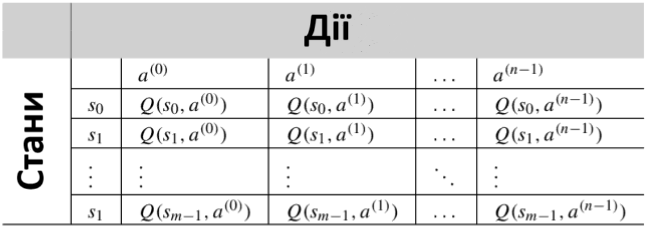
\includegraphics[scale = 1]{Pictures/QTable.png}\\
  Таблиця 2.1: Візуальне представлення Q - таблиці для середовища з \newline n станами та m діями, 
  де кортеж стан-дія педставляє Q-значення.\\
\end{center}

\par Очевидно, що побудова такої таблиці дуже дорога, якщо окремий простір дій-станів є 
великим, то він швидко стає нездійсненним для управління. 
Крім того, побудова таблиці також можлива лише тоді, коли дії є диск\-рет\-ними. Щоб вирішити цю
 проблему, ми можемо замінити Q-таблицю параметризованим апроксиматором, який можна 
 навчити за допомогою правила оновлення, подібного до \ref{eq:estimateQ}.
 Також постає проблема між дослідженням та експлуатацією, коли необхідно 
 збалансувати спроби знайти нові шляхи для підвищення ефективності та використання 
 вже відомих оптимальних стратегій. Евристики, такі як
  політика епсілон-жадібності, поєднують розвідку та експлуатацію, але задовільної 
  або однозначної відповіді на цю проблему не існує.
\par У Q-навчанні ми обираємо дію на основі її винагороди. 
Агент завжди обирає оптимальну дію. Таким чином, він генерує максимальну винагороду, 
можливу для даного стану.
При епсилон-жадібному виборі дій агент використовує як експлуатацію, 
щоб скористатися перевагами попередніх знань, так і розвідку, щоб шукати нові варіанти Рис. \ref{fig:epsilongreedy}.
\begin{figure}[H]
  \centering
  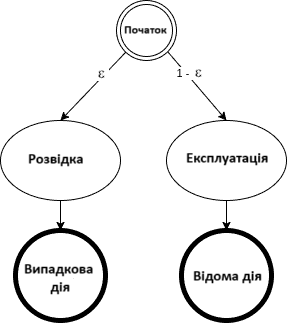
\includegraphics[scale = 1.25]{Pictures/q-learning-epsilon-greedy-1.png}
  \caption{Візуальне представлення епсилон-жадібного підходу до вибору дій.}
  \label{fig:epsilongreedy}
\end{figure}
Епсилон-жадібний підхід обирає дію з найбільшою очікуваною винагородою в більшості випадків,
 балансуючи між розвідкою та експлуатацією. Розвідка дозволяє спробувати щось нове, що іноді
  суперечить наявним знанням. З невеликою ймовірністю $\varepsilon$ ми вирішуємо 
  досліджувати, вибираючи дію випадково, незалежно від оцінок значення дії.
\subsection{Deep Q-Network}
Найпростіше покращення, яке глибокі нейронні мережі (DNN) можуть запропонувати
 для Q-навчання, - це діяти як апроксиматори Q-значення замість дорогої 
 Q-таблиці. DNN може спостерігати за поточним станом і можливою дією та 
 безпосередньо наближати значення Q. Це має очевидну перевагу в тому, що 
 нейронна мережа здатна узагальнювати наявні пари стан-дія. Завдяки здатності
  до узагальнення, агент, який використовує глибоке Q-навчання, може точно 
  визначати значення стану-дії для рідкісних або раніше небачених комбінацій 
  стану-дії.
  \par Нейронна мережа, що використовується для прогнозування Q-значень кожної дії стану, може бути використана в 
  поєднанні з політикою $\varepsilon$-жадібності для випадкового та жадібного дослідження
  середовища та навчання DQN з можливістю прогнозування значень дій стану.
  \begin{figure}[H]
    \centering
    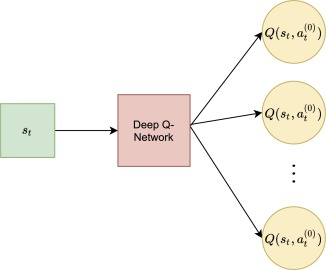
\includegraphics[scale = 1]{Pictures/DQN.jpg}
    \caption{Обчислення значень стан-дія для всіх можливих дій одного стану за один прохід.}
    \label{fig:DQN}
  \end{figure}

  Для тренування DQN спочатку відбирають зразки середовища, щоб зібрати "досвід". Ці 
  вибірки досвіду називаються епізодами і додаються до пам'яті відтворення, яка черпає
   натхнення з психологічних досліджень.\\ Щоб оновити оцінку Q-значення, епізоди 
   витягуються з пам'яті відтворення і функція втрат, отримана з \ref{eq:loss}, обчислюється як

   \bql{eq:loss} L_{s, a, r, s'} = (r + \gamma \max_{a'}Q(s',a') - Q(s,a))^2, \eq

  \noindent де $s'$ стан, до якого агент потрапив після виконання дії a у стані s. У втратах ми припускаємо,
   що оцінка Q-значення базується на виборі оптимальних дій, тому максимальне значення стан-дія 
    з можливих дій використовується як значення наступного стану. Градієнт функції втрат поширюється
     через DQN оновлюючи його ваги, поступово покращуючи прогнози значення Q. Як зазвичай для
      нейронних мереж, функція втрат застосовується до партії з декількох переходів, а потім 
      усереднюється для покращення точності градієнтів.

\section{Advantage Actor-Critic (A2C)}
Алгоритм {\em актор-критик} - це тип алгоритму навчання з підкріпленням, який поєднує в собі аспекти методів, 
що базуються на політиці (актор) та ціннос\-тях (критик). Цей гібридний підхід призначений для усунення 
обмежень кожного методу при використанні окремо.

У рамках акторно-критичного підходу агент ({\em актор}) вивчає політику для прийняття рішень, а 
ціннісна функція ({\em критик}) оцінює дії, здійснені актором.

Одночасно критик оцінює ці дії, визначаючи їхню цінність або якість. Ця подвійна роль 
дозволяє методу досягти балансу між розвідкою та експ\-луа\-тацією, використовуючи сильні сторони як 
політичної, так і ціннісної функцій.

\subsection{Актор}
  Актори вивчають параметризовані політики $\pi_{\theta}$, використовуючи градієнт політики, як показано у рівнянні \ref{eq:actor} доведення якого описано в \cite{Ch3}.
  \bql{eq:actor} \nabla_{\theta}J(\theta) = \mathbb{E}[A_{t}^{\pi}\nabla_{\theta} \log \pi_{\theta}(a_t,s_t)], \eq
де $A_{t}^{\pi}$ - {\em перевага} яку генерує критик.
Актор вибирає дії на основі поточної політики, взаємодіючи з середовищем і збираючи дані про свої дії та
отримані винагороди. Потім актор оновлює параметри політики, щоб покращити її відповідно до обчисленого 
градієнта, з метою максимізації довгострокового виграшу.
\subsection{Критик}
Як вже було сказано вище, критики в свою чергу відповідають за те, щоб навчитися оцінювати пари 
(s; a) і використовувати це для отримання $A^{\pi}$

Інтуїтивно зрозуміло, що {\em функція переваги} $A^{\pi}(s_t,a_t)$ вимірює ступінь, до якого дія є кращою або 
гіршою за середню дію політики в конерутному стані. Перевага визначається рівнянням \ref{eq:advantage}.
\bql{eq:advantage} A^{\pi}(s_t,a_t) = Q^{\pi}(s_t,a_t) - V^{\pi}(s_t). \eq \\
Загальний алгоритм A2C виглядає наступним чином:
\begin{enumerate}
  \item \emph{Ініціалізація}: 
  \begin{itemize}
      \item Ініціалізувати параметри актора (політики), та параметри критика (функції значення).
  \end{itemize}
  
  \item \emph{Взаємодія з середовищем}:
  \begin{itemize}
      \item Агент взаємодіє з середовищем, вибираючи дії відповідно до поточної політики, визначеної актором.
      \item Середовище надає спостереження про стан та винагороди у відповідь на дії агента.
  \end{itemize}
  
  \item \emph{Обчислення переваги}:
  \begin{itemize}
      \item Обчислити функцію переваги $A^{\pi}(s,a)$ на основі поточної політики та оцінених значень станів.
      \item Функція переваги кількісно характеризує перевагу виконання певної дії в певному стані порівняно з середнім очікуваним поверненням.
  \end{itemize}
  
  \item \emph{Оновлення політики та значень}:
  \begin{itemize}

      \item \emph{Оновлення актора}: Використовуйте метод градієнта політики для оновлення параметрів актора.
      \item \emph{Оновлення критика}: Використовуйте метод на основі значень для оновлення параметрів критика. Це часто включає мінімізацію помилки тимчасової різниці (TD). 
  \end{itemize}
\end{enumerate}

\section{Проксимальна оптимізація політики(PPO)}

Проксимальна оптимізація політики (PPO) - це алгоритм навчання з підкріпленням, розроблений компанією OpenAI. 
Існують два основних типи PPO, які включають:

\begin{itemize}
    \item PPO з обмеженням (clip)
    \item PPO з використанням Kullback-Leibler Proximity (KL-PEN)
\end{itemize}

Перш ніж заглибитись у варіанти, спростимо сурогатну ціль \(J_{CPI}(\theta)\), ввівши відношення ймовірностей
 \(r_t(\theta) = \frac{\pi_{\theta}(a_t|s_t)}{\pi_{\theta_{\text{old}}}(a_t|s_t)}\) і для стислості позначимо 
 перевагу \(A_{\pi_t}^{\theta_{\text{old}}}\) як \(A_t\). Сурогатною метою стає:
\bql{eq:J_CPI}J_{CPI}(\theta) = \mathbb{E}_{\pi_{\theta_{\text{old}}}}[r_t(\theta)A_t],\eq
де сурогатна ціль - це функція, яка використовується в методах градієнта політики, 
щоб наблизити справжню цільову функцію, яка вимірює ефективність політики.

Перший варіант, PPO з адаптивним KL-штрафом, вводить до мети адаптивний KL-штрафний доданок, який має на меті 
контролювати розбіжність між новою та старою політикою. Цей штрафний член віднімається від переваги, зваженої 
на важливість, що призводить до наступної мети:
\bql{eq:J_KLPEN}J_{KLPEN}(\theta) = \max_{\theta} \mathbb{E}_t[r_t(\theta)A_t - \beta \text{KL}(\pi_{\theta}(a_t|s_t) || \pi_{\theta_{\text{old}}}(a_t|s_t))],\eq
тут \(\beta\) є адаптивним коефіцієнтом, який контролює розмір штрафу KL, змінюючи довірчу область оптимізації. 
Проблема використання постійного коефіцієнта вирішується шляхом оновлення \(\beta\) після кожного оновлення політики за 
допомогою евристичного правила оновлення.

На противагу цьому, PPO з обрізаною сурогатною метою спрощує обчислення, видаляючи обмеження KL і використовуючи 
обрізану версію сурогатної мети. Обрізана мета \(J_{CLIP}(\theta)\) визначається наступним чином:
\bql{eq:J_CLIP}J_{CLIP}(\theta) = \mathbb{E}_t[\min(r_t(\theta)A_t, \text{clip}(r_t(\theta), 1 - \epsilon, 1 + \epsilon)A_t)],\eq
де \(\epsilon\) визначає околицю відсікання, гарантуючи, що відношення ймовірностей \(r_t(\theta)\) залишається 
у визначеному діапазоні. Відсікаючи ціль, PPO запобігає великим і ризикованим оновленням політики, роблячи процес
 оптимізації безпечнішим і стабільнішим.\\

 Загальний алгоритм PPO виглядає наступним чином:
 \begin{itemize}
  \item {\em Ініціалізація мережі політики}: Ініціалізації нейронної мережі, яка представляє політику. Ця мережа приймає поточний стан на вході і виводить розподіл ймовірностей можливих дій.
  
  \item {\em Збір траєкторій}: Агент взаємодіє з навколишнім середовищем, дотримуючись поточної політики, під час якої він збирає траєкторії.
  
  \item {\em Обчислення оцінок переваг}: Використовуючи зібрані траєкторії, обчислюються оцінки переваг для кожної пари стан-дія.
  
  \item {\em Обчислення сурогатної мети}: Обчислюється сурогатна мета, яка є функцією старих і нових параметрів політики та оцінок переваг. Ця ціль апроксимує покращення політики, гарантуючи при цьому, що оновлення політики залишається в безпечному діапазоні.
  
  \item {\em Оптимізація мережі політик}: Використовується стохастичний градієнтний спуск (SGD) або інший варіант для оновлення параметрів мережі політик, мінімізуючи сурогатну мету.
\end{itemize}

\section{Середовище гри}
 \setcounter{equation}{0}
 \setcounter{theorem}{0}
 Комп’ютерні ігри надають необіхдну інформацію за допомогою екрану, тим самим забираючі
 прямий доступ до значення різних параметрів і представляючи їх у вигляді зображень. 
 Люди у свою чергу можуть легко сприймати цю інформацію, а DRL агент сприймає лише числові значення 
 параметрів гри, через це інформацію на зображенні треба 
 обробити та представити у вигляді значень, які агент може сприймати. Варто зазначити,
 що ця проб\-лема наявна лише при тренувані DRL агентів сторонім лицем, а не розробником гри.
 Так як розробники гри мають всю необхідну інформацію у числових значеннях, вони можуть інтегрувати DRL
 у їхню гру, тим самим підвищивши ефективність навчання агента.\\


Кожен кадр гри містить візуальне зображення поточного стану ігрового середовища. 
І в залежності від динаміки ігрової системи, агент має отримувати n-кількість зображень.
 Зібрані зображення потребують попередньої обробки, щоб виділити корисну інформацію 
 і зменшити обчислювальні витрати. Основні методи обробки зображень включають:
 \begin{itemize}
  \item \emph{Зменшення роздільної здатності:} Висока роздільна здатність зображень 
  може значно збільшити обчислювальні витрати. Тому, зображення часто 
  зменшуються до меншого розміру.
  \item \emph{Перетворення в градації сірого:} Перетворення зображень у градації 
  сірого зменшує кількість каналів, що знижує обчислювальну 
  складність.
  \item \emph{Нормалізація:} Піксельні значення зображень нормалізуються до діапазону 
  [-1, 1]. Це підвищує швидкість навчання та впроваджує незалежність відносно розширення екрану.
  \item \emph{Обтинання:} Деякі частини зображення, такі як інтерфейс користувача 
  (UI), можуть не містити корисної інформації для алгоритмів DRL.
  \end{itemize}
  Після попередньої обробки зображення можуть бути піддані подальшій обробці з 
  використанням методів комп'ютерного зору для виділення ключової інформації:
  \begin{itemize}
    \item \emph{Виявлення об'єктів:} Використовуючи алгоритми, такі як YOLO 
    (You Only Look Once) або Faster R-CNN, можна виявити та ідентифікувати ключові 
    об'єкти на зображенні, наприклад, персонажів, ворогів, предмети і т.д.
    \item \emph{Сегментація зображень:} Методи сегментації дозволяють розділити 
    зображення на області, що відповідають різним об'єктам чи частинам сцени.
\item \emph{Відстеження об'єктів:} Методи відстеження об'єктів дозволяють виз\-начити 
траєкторії руху об'єктів у часі, що є важливим для розуміння динаміки ігрового 
середовища і прогнозування майбутніх станів.
\end{itemize}

Після обробки зображень, їх необхідно перетворити у формат, зручний для алгоритмів DRL:
\begin{itemize}
\item \emph{Тензорне представлення:} Зображення перетворюються у тензори, 
які можуть бути подані на вхід нейронних мереж. Наприклад, тензор для зображення 84x84 
у градаціях сірого матиме розмір 84x84x1.
\item \emph{Векторні ознаки:} Крім зображень, важливо представити інші ознаки, такі 
як позиції об'єктів, стан здоров'я персонажа, наявні ресурси тощо. Ці дані можуть бути
 представлені у вигляді векторів і об'єднані з тензорами зображень.
\end{itemize}
Таке подання інформації про стан гри відповідає вимогам і можливостям алгоритмів 
глибокого навчання з підкріпленням, забезпечуючи їм доступ до повної та релевантної 
інформації для ефективного тренування або прийнят\-тя рішень у грі.